\documentclass[a4paper, 12pt, ngerman, titlepage]{scrartcl} % a4paper, damit nicht amerik. letterpaper; 12pt Schriftgröße; ngerman Umlaute äöü oder sowas; titlepage damit keine Seitenzahl bei Titelseite, \subject etc. dazugeknallt werden können, hübscher isses auch; scratrcl soll deutsch und hübsch sein, hat aber keine chapter nur section, aber chapter fangen auch neue Seiten an https://texwelt.de/fragen/15869/seitennummer-in-scrartcl-auf-titelseite-unterdrucken
% hatte bis 2025-05-14 a4paper in [] nach springer nature vorlage habe ich da mal pdflatex reingeschrieben, scheint nix kaputt zu machen. Ich glaube KOMA script mit scrartcl sollte sich schon um DIN A4 kümmern
\usepackage[utf8]{inputenc} % moderner Zeichencode, auch mit ä ö ü und so'n Kram
\usepackage{lmodern} % hübsche Schrift? hab's vergessen
\usepackage[T1]{fontenc} % Schriftarten gute diese glaube ich
\usepackage[onehalfspacing]{setspace} % Zeilenanbstand, Grüße ans Kompendium
\usepackage[ngerman]{babel} % Sprache, ngerman Silbentrennung nach neuer Rechtschreibung und so
% \usepackage{verbatim} % das habe ich gefunden um ganze Blöcke inklusive Zeilenumbrüchen auszukommentieren -- Nachtrag lol, bullshit, verbatim direkt druckt code ohne auszuführen
% \usepackage[normalem]{ulem} % zum Durchstreichen https://texwelt.de/fragen/3223/wie-kann-ich-text-durchstreichen ulem besser wegen äöüß und neuer. soul besser als ulem für Zeilenumbrüche, Zeilenumbrüche bei Links waren nicht existent mit ulem https://tex.stackexchange.com/questions/74893/strikeout-when-which-package-ulem-vs-soul-vs#comment710882_74910 ich versuche also ulem mit normalem als Option https://golatex.de/viewtopic.php?t=3079 prima, scheint zu klappen

% \usepackage{acronym} % added 2024-06-05 https://www.heise.de/tipps-tricks/Abkuerzungsverzeichnis-in-LaTeX-erstellen-4982473.html oder https://de.wikibooks.org/wiki/LaTeX-W%C3%B6rterbuch:_Abk%C3%BCrzungsverzeichnis wiki empfiehlt womöglich package glossaries, hab da gerade kein Bock zu, acronym tut's bestimmt auch https://www.overleaf.com/learn/latex/Glossaries
% printonlyused could be put in []
% [v2 used because compile time in overleaf free]
% I try \usepackage{glossaries} 2025-06-03


\usepackage{geometry} % Seitenränder, ein wahrer Krampf
\geometry{left=30mm, right=30mm, top=25mm, bottom=25mm} % mm besser als cm, bestimmt wegen , und . als Dezimaltrennzeichen, der Krampf hat sich entspannt, mm rulez
\usepackage[autostyle=true, german]{csquotes} % für Anführungszeichen in Zitaten in versch. Sprachen und so: https://www.namsu.de/Extra/pakete/Csquotes.html

\usepackage[backend=biber, style=authoryear-icomp, bibstyle=authoryear, dashed=false, maxcitenames=2, maxbibnames=99, block=none]{biblatex} % Zitationsstil, authoryear kommt Harvard nah -- date=year von Antwort aus https://texwelt.de/fragen/27027/zitationsstil-anpassen-biblatex-authoryear
% 2025-04-22 block=nbpar wäre erklärt bei Seite 51 von der Anleitung 3.1.2.1 https://mirrors.ibiblio.org/CTAN/info/translations/biblatex/de/biblatex-de-Benutzerhandbuch.pdf

\addbibresource{references.bib} %Bibliographie erstellen
% wenn unter Zitation -> Latex Assistant F7 ausgegraut, dann: Extras > Optionen > Zitation, da LaTeX anklicken
% im Moment (2022-09-06) ist TeXStudio angegeben und: quote; autocite; cite; parencite & quote; autocite; cite; parencite
% inspiriert von: https://help.citavi.com/topic/latex-assistent-kopieren
% stil authoryear-icomp s. Handbuch Seite 77 https://mirrors.ibiblio.org/CTAN/info/translations/biblatex/de/biblatex-de-Benutzerhandbuch.pdf
% 2025-04.02 maxbibnames=99 aus [] von biblatex genommen, da standard wohl =maxnames ist, Anleitung S. 49... Ok, doch nicht, gibt dann Fehler. vierlleicht lieber =99, weil ich die Schrägstriche definiert habe? Und sorting=nyt etnfernt, sollte Standard sein. Und dashed=false hinzugefügt Anleitung zu bibtex S. 81 bei Bibliographiestile
% hier steht auch maxbibnames=99 ist beste: https://tex.stackexchange.com/questions/12806/guidelines-for-customizing-biblatex-styles

% erst Nachname, dann Vorname https://www.mrunix.de/forums/showthread.php?75128-Biblatex-Nachname-Vorname klappt nur leider auch mit family-given nicht 2025-04-02 \DeclareNameAlias{default}{family-given}
% 2025-04-02 ohne ist nur beim ersten in der Bibliography der Nachname zu Beginn, danach ist es Vorname Nachname 

% https://texwelt.de/fragen/29060/biblatex-nachname-vorname default durch author (und editor und translator) ersetzt
\DeclareNameAlias{author}{family-given} % 2025-05-28 scheint nur author zu ändern, bei editor bleibts, daher: 
\DeclareNameAlias{editor}{family-given}
% \DeclareNameAlias{editor}{sortname}
% \DeclareNameAlias{translator}{sortname}


%%%%%%%%%%%%%%%% %%%%%%%%%%%%%%%% %%%%%%%%%%%%%%%% 
%%% von copilot für prompt: 
% wie verändere ich textcite in biblatex so, dass alle namen mit komma und und aufgezählt werden?
% \DeclareDelimFormat{andothersdelim}{\addcomma\space}
% \DeclareDelimFormat{finalnamedelim}{\space und\space}
% \DeclareDelimFormat{multinamedelim}{\addcomma\space}
%scheint aber nix zu ändern 2025-05-28

%%% von copilot für prompt: 
% das hat noch nicht geklappt. ich nuze folgenden stil: \usepackage[backend=biber, style=authoryear-icomp, bibstyle=authoryear, dashed=false, maxcitenames=2, maxbibnames=99]{biblatex}
% \DeclareDelimFormat{finalnamedelim}{\space und\space}
% \DeclareDelimFormat{multinamedelim}{\addcomma\space}
%scheint aber nix zu ändern 2025-05-28
%%%%%%%%%%%%%%%% %%%%%%%%%%%%%%%% %%%%%%%%%%%%%%%% 


\DefineBibliographyStrings{ngerman}{
   andothers = {{et\,al\adddot}},
} % damit wird u.a. zu et al. siehe https://tex.stackexchange.com/questions/236854/changing-u-a-of-german-to-et-al

% no p. pp. and : instead of ,
% https://stackoverflow.com/questions/58448860/how-can-i-add-colons-and-remove-p-pp-from-in-text-citations-with-biblatex
\DefineBibliographyStrings{ngerman}{
  page             = {},
  pages            = {},
}  % ich habe german anstatt english ergänzt % 2025-05-27 auf ngmerman geändert
% colon instead of comma bei in text cite
\renewcommand{\postnotedelim}{\addcolon \addspace} % \addspace kommt von mir

% no p.von anderer Quelle
% \DeclareFieldFormat{postnote}{#1}
% \DeclareFieldFormat{multipostnote}{#1}

\renewcommand*{\multinamedelim}{\addslash}
\renewcommand*{\finalnamedelim}{\multinamedelim}
% Schrägstriche zur Abtrennung https://golatex.de/viewtopic.php?t=18487 andere Quelle (hat nicht auf Anhieb funktioniert) https://groups.google.com/g/de.comp.text.tex/c/eSVMHAMphCA

%%%%%%% danke copilot
% Spezielle Anpassung für textcite
\DeclareDelimFormat[textcite]{finalnamedelim}{\space und\space}
\DeclareDelimFormat[textcite]{multinamedelim}{\addcomma\space}
%%%%%%%%%%%%%

% doppelte Nachnamen wegen shorthands (auto. durch citavi erstellt) in den refenerces.bib https://golatex.de/viewtopic.php?t=13563
% keine KURZBELEGE in CITAVI für Harvard Zit. verwenden!! https://www1.citavi.com/sub/manual6/de/index.html?cse_customizing_citation_keys.html

% \usepackage{minitoc} %h Mini Inhaltsverzeichnis https://cs.brown.edu/about/system/managed/latex/doc/minitoc.pdf
% \usepackage{pdfpages} % vielleicht mal pdfs direkt hier als anhang einbinden https://texwelt.de/fragen/19153/pdf-dateien-in-anhang-einbinden-aber-formatierung-des-vorhergehenden-dokuments-ubernehmen
% \usepackage{subfiles} % Best loaded last in the preamble https://de.overleaf.com/learn/latex/Multi-file_LaTeX_projects%23The_subfiles_package


%%%%%%%%%%%%%%%%%%%%%%%%%%%%%%%%%%%%%%%%%%%%%%%%%%%%
\usepackage{graphicx}   % PDF Support % vorher war hier auch [pdftex] eingebunden. Nachdem ich hyperref in der Präambel nach unten geschoben habe, hat overleaf aber einen Fehler ausgespuckt
\usepackage[hidelinks]{hyperref}   % Hyperlinks % hidelinks keine bunten Kasten um klickbare Elemente: https://texwelt.de/fragen/1121/wie-entferne-ich-die-roten-rahmen-um-hyperlinks? 2025-05-14
\usepackage{times}              % Font fuer PDF besser
\usepackage{thumbpdf}           % PDF Thumbnails erstellen
% https://www.linux-community.de/ausgaben/linuxuser/2005/04/mit-pdflatex-bessere-pdf-dateien-erzeugen/2/  
% 2025-05-14
%%%%%%%%%%%%%%%%%%%%%%%%%%%%%%%%%%%%%%%%%%%%%%%%%%%%

\subject{Universität Bremen\\ Sommersemester 2025\\ Masterarbeit}
\title{Chancen und Risiken von Fremdmaterial: Eine beispielhafte Analyse und Wertung von Unterrichtsmaterial der Arbeitnehmerkammer Bremen für den Politikunterricht an berufsbildenden Schulen in Bremen.} 
%%%%%%%%%%%%% TitelBRainStorming %%%%%%%%%%%%%%%%%%%%%%%%%
% Nutzung von fremden Unterrichtsmaterialien. Eine exemplarische Analyse für den Politikunterricht an berufsbildenden Schulen in Bremen
% Nutzung von Unterrichtsmaterialien einer externen Institution. Eine exemplarische Analyse für den Politikunterricht an berufsbildenden Schulen in Bremen

% Entwürfe 2025-03-04 Di.
% Nutzung von fremden Unterrichtsmaterialien. Eine exemplarische Analyse für den Politikunterricht an berufsbildenden Schulen in Bremen

% Analyse und Wertung von großflächig angelegtem Unterrichtsmaterial Materialvorlagen: Exemplarisches Vorgehen mit Material der Arbeitnehmerkammer Bremen.

% Analyse und Wertung von Materialvorlagen für den Politikunterricht an berufsbildenden Schulen in Bremen: Eine beispielhafte Analyse mit Material der Arbeitnehmerkammer Bremen.

% Gekürzt:
% Analyse und Wertung von Materialvorlagen: Eine beispielhafte Analyse anhand von Unterrichtsmaterial für den Politikunterricht an berufsbildenden Schulen in Bremen der Arbeitnehmerkammer Bremen.

% Die Realität der Nutzung von institutionellem Unterrichtsmaterial entgegen selbsterstelltem Material: Eine beispielhafte Analyse anhand von Unterrichtsmaterial der Arbeitnehmerkammer Bremen für den Politikunterricht an berufsbildenden Schulen in Bremen.

% Nur selbsterstelltes Unterrichtsmaterial? Chancen und Risiken von Fremdmaterial: Eine beispielhafte Analyse und Wertung von Unterrichtsmaterial der Arbeitnehmerkammer Bremen für den Politikunterricht an berufsbildenden Schulen in Bremen.

% Unterricht von der Stange? Chancen und Risiken von Fremdmaterial: Eine beispielhafte Analyse und Wertung von Unterrichtsmaterial der Arbeitnehmerkammer Bremen für den Politikunterricht an berufsbildenden Schulen in Bremen

% Kriterien zur Bewertung von externen Unterrichtsmaterialien im Politikunterricht. Am Beispiel 
% Geschenke nimmt man gerne an
% Unterricht von der Stange
% Erleichterung durch fertiges Unterrichtsmaterial
%%%%%%%%%%%%%%%%%%%%%%
\author{Paul Aljoscha Klein\\ $\#$ 4134166\\ $\ast$ 20.07.1995\\ \\ Erstprüfer: Prof. Dr. Andreas Klee \\ Zweitprüferin: Dr. Eva Anslinger}
\date{Juli 2025}
% So sieht's gut aus mit titlepage bei Dokumentklasse


\usepackage[xindy, toc, acronym]{glossaries}
% xindy weil: https://tex.stackexchange.com/questions/199211/differences-between-xindy-and-makeindex/199841#199841
% https://en.wikibooks.org/wiki/LaTeX/Glossary#cite_note-2
\makeglossaries % das makeglossaries muss vor \begin{document} stehen, damit es funktioniert

    \newacronym{abs}{Abs.}{Abschnitt}
    \newacronym{ank}{ANK}{Arbeitnehmerkammer Bremen}
    \newacronym{bbk}{BBK}{Beutelsbacher Konsens}
    \newacronym{bpb}{bpb}{Bundeszentrale für politische Bildung}
    \newacronym{bzw}{bzw.}{beziehungsweise}
    \newacronym{c}{\copyright}{Copyright}
    \newacronym{doi}{DOI}{Digital Object Identifier}
    \newacronym{ebd}{ebd.}{ebenda}
    \newacronym{etc}{etc.}{et cetera}
    \newacronym{gp}{GP oder GuP}{Gesellschaft und Politik}
    \newacronym{gpje}{GPJE}{Gesellschaft für Politikdidaktik und politische Jugend- und Erwachsenenbildung}
    \newacronym{lis}{LIS}{Landesinstitut für Schule}
    \newacronym{nw}{NW}{Naturwissenschaften}
    \newacronym{oä}{o.Ä.}{oder Ähnliche(s)}
    \newacronym{s}{s.}{siehe}
    \newacronym{S}{S.}{Seite}
    \newacronym{suub}{SuUB}{Staats- und Universitätsbibliothek Bremen}
    \newacronym{sek}{SEK}{Sekundarstufe}
    \newacronym{sus}{SuS}{Schülerinnen und Schüler}
    \newacronym{ua}{u.A.}{unter Anderem}
    \newacronym{url}{URL}{Universal Ressource Locator }% (einheitlicher Ressourcen Verorter, Webadressen)
    \newacronym{vgl}{vgl.}{vergleiche}
    \newacronym{wuk}{WUK}{Welt-Umweltkunde}
    \newacronym{zap}{zap}{Zentrum für Arbeit und Politik}
    \newacronym{zb}{z.B.}{zum Beispiel}

\begin{document}
% \maketitle
% \thispagestyle{empty}
% \pagestyle{empty} war für Seitennummer weg in Klasse article
\pagenumbering{roman}
\addsec{Abstract}
blub
\newpage
\tableofcontents % war früher mal vor pagenumbering. Macht das einen Unterschied? Keine AHnung 2024-06-05 ah ja, will ja nicht das Inhaltsverzeichnis Seitenummeriert haben 2024-06-06

\clearpage
\newpage
% \addsec{Abkürzungsverzeichnis}

\printglossary[type=\acronymtype, title={Abkürzungsverzeichnis}, toctitle={Abkürzungsverzeichnis}, nonumberlist] % Acronymtype ist von glossaries, title und toctitle sind Titel im Inhaltsverzeichnis

\clearpage
\newpage

\setcounter{page}{1}
\pagenumbering{arabic}

\section{Einleitung \& Theoretischer Hintergrund}
% Unterrichtsmaterial kommt nicht nur aus Schulbüchern oder wird von den Lehrkräften selbst erstellt

\subsection{Von der Theorie in die Praxis} \label{theorie in praxis}
Es gibt extensive Forschung in den Erziehungswissenschaften und der Fachdidaktik. Insbesondere der Bereich der politischen Bildung ist darüber hinaus mit zahlreichen interdisziplinären Brücken in die Sozialwissenschaften und über einen schulischen Bildungsbegriff hinaus ein Forschungsfeld, welches in seiner Gänze nicht einmal von Menschen zu überblicken ist, die ihr ganzes (Arbeits-)Leben der politischen Bildung gewidmet haben. 

Gleichzeitig sind sowohl die Möglichkeiten zur weiteren Erforschung als auch der konkrete Forschungsbedarf im Detail von nicht zu überblickender Größe. 
% explizit einschließt, dass mindestens genauso viel unerforscht ist und vieles sicherlich sinnvoll wäre zu erforschen. 

In unserer hochkomplexen Welt gilt dies sicherlich für das Gros an Forschungsbereichen. Die Eingrenzung und damit Abgrenzung von Forschungsgegenständen ist daher stets zwangsläufiger Bestandteil des Forschens. In der Praxis bedeutet das, immer wieder aushandeln zu müssen, inwieweit Querverbindungen zu anderen Bereichen notwendig sind und an welcher Stelle der Fokus wieder auf das Wesentliche zu legen ist.
Diese Entscheidungen sind optimalerweise logisch zu begründen. Getroffen werden müssen sie dennoch. Das ist sicherlich mit Arbeit verbunden. 

Analog zu den Entscheidungen, die Forschende treffen müssen, um handlungsfähig zu sein, das heißt fokussiert ihre Forschung vorantreiben zu können, ist die Eingrenzung eines Lerngegenstandes ebenfalls zu begründen und mit Entscheidungen verbunden. 
Lehrende befinden sich diesbezüglich also in einer ähnlichen Situation wie Forschende. 

Es ließe sich allerdings argumentieren, dass die Notwendigkeit im Unterrichten von Weltwissen Entscheidungen zu treffen -- wie es im Schulkontext stattfindet -- auf einer vageren Datengrundlage stattfinden muss. In der Forschung wird sich wegen der zuvor beschriebenen Notwendigkeit der Eingrenzung zunehmend spezialisiert. Im schulischen Weltverstehen-Lernen hingegen ist in weiten Teilen (noch) kein hochspezialisiertes Verständnis gefordert. Stattdessen steht ein allgemeines Zusammenhänge-verstehen-Lernen im Vordergrund. Das setzt Lernen an exemplarischen Lerngegenständen voraus. 
Dies gilt insbesondere für die politische Bildung -- nicht nur in allgemeinbildenden Schulen, sondern auch für Politikunterricht in der dualen Berufsbildung \autocite[vgl. \gls{abs} \ref{bplan}; \gls{S} \pageref{bplan} \&][4; 9-13]{bplan}.
In der Ausbildung zum Lehramt wird Wert darauf gelegt, solche Entscheidungen, welche Lerngegenstände ausgewählt werden, umfassend begründen zu können. 
In der Praxis des Lehrens wird Wert darauf gelegt, tatsächlich zu unterrichten.
In der wissenschaftlichen Literatur wurde dieses ständige im Widerspruch stehen, dem Lehrkräfte an verschiedenen Stellen ausgesetzt sind, längst erkannt und jener als Antinomie bezeichnet \autocite[\gls{vgl} \gls{zb}][]{Helsper.2001}.

Den kompletten Wissensstand der unterrichteten Domäne von einzelnen Lehrkräften fachwissenschaftlich oder didaktisch im kompletten Überblick zu behalten, ohne dass Teile des Alltagsgeschäfts hintenüber fallen, erschiene daher eine utopische Forderung.

Daher ist es eine willkommene Abwechslung, in dieser Arbeit zwar nicht zur Erleichterung des Handwerks des Unterrichtens beizutragen, wohl aber eine Initiative zum Untersuchungsgegenstand zu haben, der genau diese Intention unterstellt werden kann. 

\subsection{Lerngegenstände}
Unterrichten an Bildungsinstitutionen passiert meist unter Zuhilfenahme von Medien und die Planung ist im besten Fall verschriftlicht oder anderweitig aufgezeichnet, \gls{zb} durch Grafiken. Die Planung des Unterrichts und die Auswahl oder Erstellung der zum Unterrichten verwendeten Materialien nehmen dabei einen erheblichen Zeitaufwand seitens der Lehrkräfte ein.

Das Zurückgreifen auf bestehende Medien ist dabei natürlicher Bestandteil des Lernens. So ist die (Primär-)Quellenanalyse im Geschichtsunterricht, das Lesen eines Haikus in Deutsch, die Analyse einer Inszenierung, das Basteln an einem Motor oder das Erhitzen von Chemikalien alles die natürliche Benutzung von Unterrichtsmaterial. 

Um diversen Gegebenheiten gerecht zu werden, ist das Material jedoch häufig abstrahiert. Eine Dampfmaschine steht womöglich nicht zur Verfügung. In so einem Fall kann \gls{zb} auf eine Explosionszeichnung, einen Film, ein Modell oder eine Beschreibung zurückgegriffen werden. Eine Beschreibung in Worten erfordert dabei eine höhere Abstraktionsebene als ein Modell und birgt die Gefahr, schlechtere Lernergebnisse zu erzielen; was dann durch entsprechende Einbettung oder die Ergänzung weiterer Materialien, wie einem Schema oder einem Film, versucht werden sollte zu kompensieren. Wie anhand dieses Beispiels bereits deutlich wird, erfordert bereits die Auswahl der Lehrmaterialien Arbeit, bevor überhaupt mit den Lernenden in Interaktion getreten wird. 
Wenn nun in der politischen Bildung eine Rede analysiert wird, sind die naheliegenden Möglichkeiten überschaubar. Eine Verschriftlichung und eine Videoaufnahme bieten sich an. 

Gerade in der politischen Bildung liegt der Lerngegenstand jedoch häufig auf noch ferner liegenden Abstraktionsebenen. Es geht um hochkomplexe Konzepte, die in der physischen Welt schwer greifbar sind. Entsprechend viele nah- und fernliegende Möglichkeiten bestehen bei der Auswahl an Unterrichtsmaterial\footnote{Das soll nicht bedeuten, dass die Vorbereitungen im Mathematikunterricht zum ergänzenden Material einer eindeutigen Rechenaufgabe, \gls{zb} durch kleinschrittiges Vorgehen, grafische Darstellung oder Darstellungen in der physischen Welt, nicht ebenfalls hochkomplex sind und zahlreiche Entscheidungen erfordern. Aber viele Lerngegenstände der politischen Bildung sind an sich schon derart abstrahiert, dass dort die Beschäftigung mit der Darstellung unvermeidlich ist.}.

Unterrichtsmaterial, für welches bereits Entscheidungen bezüglich des exemplarischen Lerngegenstandes und der didaktischen Reduktion getroffen wurden, hat also gewaltiges Potential, eine Arbeitserleichterung darzustellen.
Beispielsweise indem es für die Zielgruppe und die Zielvorgaben aus einem Lernplan bereits vorausgewählt und für eine ansprechende Darstellung aufbereitet wurde.
Arbeit zieht jedoch auch vorgefertigtes Material nach sich, da die Beurteilung der Qualität und die Eignung sowie die Anpassung für die Lerngruppe keine Selbstverständlichkeit sind.

\subsubsection{Herkunft der Lerngegenstände}
Die Notwendigkeit des Lernens, eben auch Lerngegenstände zu haben, hat entsprechend auch verschiedene Akteure mit unterschiedlichen Intentionen auf den Plan gerufen, welche Unterrichtsmaterial feilbieten.
Einsteigend hervorzuheben sind dabei die privatwirtschaftlichen Schulbuchverlage, welche dem klassischen Bild von Unterrichtsmaterial entsprechen. Jedoch haben auch andere Institutionen das Potenzial einer Einflussnahme auf Lernende durch 
% geschickt gestaltetes 
Material entdeckt. Wirtschaftsverbänden oder großen Unternehmen kann dabei bisweilen eine andere Intention als eine altruistische unterstellt werden, die durch auf den ersten Blick kostenfreies Material verfolgt wird. So braucht man in der Forschung von Reinhold Hedtke bisweilen nicht weiter als bis zu den römischen Zahlen zu lesen, um darauf gestoßen zu werden, dass Schulen \enquote{sich zunehmend gegen weltanschauliches, wissenschaftliches, wirtschaftliches und politisches Lobbying aus Unternehmen und ihrem Umfeld wehren} müssen \autocite[i]{Hedtke2016}. 


Auch die \gls{ank} entwickelt in Kooperation mit dem \gls{zap} an der Universität Bremen Unterrichtsmaterial für den Politikunterricht.


In dieser Arbeit soll ein Versuch unternommen werden, dieses Unterrichtsmaterial zu analysieren und zu bewerten. % welches den Lehrkräften von dem quasi staatlichen Akteur der Arbeitnehmerkammer Bremen zur Verfügung gestellt wird. 






\section{Theoretischer Hintergrund / Begriffsklärungen}
Um das Material zu analysieren, hilft es mehrere Begriffe zu klären. Zum ersten eine Definition, was unter Unterrichtsmaterial verstanden werden soll und.... % Zum zweiten ein Überblick, wie politische Bildung an Berufsschulen in Bremen stattfindet. 
Dann sollen der Bildungsplan in Politik vorgestellt werden, sowie der \gls{bbk}, auf den jener Bezug nimmt. Um im späteren Verlauf die verschiedenen Lebensweltbezüge aufzeigen zu können, soll daraufhin noch die Zielgruppe der Lernenden umrissen werden. 
Blub blub, nur ausführen was die Überschriften weshalb sagen........




% fick dich, ich bin Krebs 

\subsection{Politische Bildung an berufsbildenden Schulen in Bremen}


\subsection{Bremer Bildungsplan \& Kompetenzen in der politischen Bildung} \label{bplan}
Der aktuelle Bremer Bildungsplan für politische Bildung\footnote{Als Fach vom \gls{lis} nur als Politik bezeichnet} für berufsbildende Schulen ist mit der Erscheinung \citeyear{bplan} (\citeauthor{bplan}) vergleichsweise aktuell. Die Bremer Bildungspläne für die \gls{sek} I und II der allgemeinbildenden Schulen sind alle etwa im vorletzten Jahrzehnt, zwischen \citeyear{vogel2006gy} \autocites{vogel2006gs, vogel2006gy, lower2008} und \citeyear{vogel2010gp} \autocite{vogel2010gp}, erschienen. Die Fächerbezeichnungen sind innerhalb der Bremer Bildungspläne nicht kongruent. Die unstete Bezeichnung der Fächer -- welche politische Bildung, häufig neben anderen Bereichen, mit abdecken -- wird in \gls{abs} \ref{polBildung} (\gls{S} \pageref{polBildung}) weiter diskutiert.

Politik ist neben Deutsch im Jahr 2024/2025 aktuell das einzige andere Fach im Land Bremen, welches für den berufsbildenden Bereich fächerübergreifend für alle Schülerinnen und Schüler unterrichtet wird (vgl. Website des \gls{lis} \citeyear{LisBildungspläne}). Direkt im Bildungsplan \autocite[][4]{bplan} wird darauf eingegangen, dass zwar an \enquote{heterogene[...] Voraussetzungen der Schüler:innen} angeknüpft wird, was auch \enquote{die Unterschiedlichkeit der jeweiligen Bildungsgänge} berücksichtigen soll, aber als Teil der \enquote{allgemeinbildenden Fächer} sollen die \enquote{Zielsetzungen politische Urteilsfähigkeit, politische Handlungsfähigkeit und methodische Fähigkeiten} immer die Grundlage bilden. 


Allgemeine politische Kompetenzen sind die hauptsächlichen Ziele \autocite[9-13]{bplan}.

Für die \enquote{Kompetenzdimensionen in der politischen Bildung} orientiert sich der Bildungsplan stark an den Ausarbeitungen der \gls{gpje}.
Da in dieser Arbeit (\gls{s} \gls{abs} \ref{öffi}; \gls{S} \pageref{öffi}) auch auf die Verfügbarkeit und Nutzfreundlichkeit von Unterrichtsmaterial eingegangen wird, bietet es sich an, an dieser Stelle ein strukturelles Einzelfallbeispiel aufzuziehen:

\subsubsection{Exkurs: Schlechte Quellenangaben und miese Vorbildfunktion. Beginnt Medienkompetenz im Bildungsplan?} \label{gpje}
Der Bildungsplan selbst ist von fiskalisch finanzierten Stellen erarbeitet und für einen Bildungsbereich veröffentlicht, welcher sich vermutlich auch als öffentlich, sowohl in Form von öffentlichen Geldern finanziert als auch in Form von öffentlich zugänglich versteht, da es sich um einen verbreiteten, staatlich vorgezeichneten \mbox{(Weiter-)Bildungsweg} % \mbox trennt Begriff nicht 
handelt. Der Bildungsplan ist auf der Website des \gls{lis} (\citeyear[]{LisBildungspläne}) auch öffentlich zugänglich im etablierten .pdf-Format vorzufinden und bietet allen Menschen die Möglichkeit, mit diesem öffentlich erarbeiteten Wissen zu arbeiten.
Soweit erscheint das Vorgehen kohärent und sinnvoll.

Der Bildungsplan orientiert sich \gls{ua} an den Bildungsstandards der \gls{gpje}. Konkret wird das \gls{ua} Fußnote 13 im Bildungsplan \autocite[][9]{bplan} deutlich, vergleichbar zu folgender Fußnote\footnote{http://gpje.de/wp-content/uploads/2017/01/Bildungsstandards-1.pdf}. Da der perfekte Zitierstil nicht nur kontextabhängig, sondern subjektiv ist, soll dahingehend keine Wertung stattfinden. Allerdings sind an dieser Stelle bereits mehrere zitierstilübergreifende Grundsätze missachtet worden. Sich dafür zu entscheiden, einen Fußnotenzitierstil zu nutzen und an späterer Stelle ein komplettes Quellenverzeichnis, wäre eine solide Wahl. Auch wenn als dabei übliche Kurzform in der Fußnote ausschließlich einen kompletten Weblink anzugeben, schon wild ist. Nur dass es kein komplettes Quellenverzeichnis gibt.  
Es gilt, ausreichend Informationen (lieber eine zu viel als eine zu wenig) zum Auffinden anzugeben, insbesondere und mindestens Äquivalente zu Autor*innen oder Herausgeber*innen, sowie Erscheinungsjahr und Titel, sowie ein Zugriffsdatum, falls Weblinks angegeben sind. 
Als findige*r Konsument*in von Text lassen sich nun Teile von Titel und Namen sowie das Akronym der Herausgebenden im Link herauslesen. Allerdings führt der Link im Mai 2025 auf eine weiße Seite und ist damit ein Paradebeispiel, weshalb \gls{ua} wenigstens ein Zugriffsdatum angegeben sein sollte.
Als bemühter Autor einer universitären Abschlussarbeit findet man jedoch unter diesem Link\footnote{https://gpje.de/publikationen/ (06.05.2025)} einen Download mit diesem Link\footnote{https://gpje.de/wp-content/uploads/2024/07/Bildungsstandards-1.pdf (05.05.2025)}, dessen \gls{url} entsprechend der Zahlen, die ein Datum darstellen könnten, womöglich eine aktuellere Version zu der im Bildungsplan \autocite[][9]{bplan} referierten verspricht. Laut Website und Untertitel, soll es sich zwar lediglich um einen Entwurf handeln. Wobei \enquote{Entwurf} sich an dieser Stelle wohl eher als Synonym für Vorschlag lesen lässt.  Das Dokument kann jedoch nach wie vor in seiner Veröffentlichungsform strukturell kritisiert werden:
\begin{itemize}
    \item Das in der \gls{url} suggerierte Datum impliziert nun eine Veröffentlichung oder Version vom Juli 2024, im Dokument selbst ist ein \gls{c} vom Wochenschau Verlag von 2004 angegeben. Es handelt sich höchstwahrscheinlich um eine Version der viel zitierten 2. Auflage von \citeyear[]{gpje2004}. Nur dass im Bildungsplan nicht ersichtlich ist, ob er sich tatsächlich auf diese Version bezieht. Höchstwahrscheinlich bezog sich die alte \gls{url} in der 2017 zu lesen ist auf dieselbe Version, wie die, welche hier mit 2024 in der \gls{url} aufgefunden wurde. 
    
    
    \item Es gibt keinen Versionsverlauf, auf der eigenen Website der \gls{gpje} ließ sich eine Version von 2017, wie die \gls{url} im Bildungsplan \autocite[][9]{bplan} suggeriert, nicht finden. Die Zahlen 2017 und 2024 scheinen in diesem Fall schlicht keine andere Version zu kennzeichnen. Denkbar ist, dass es nur intern erneut hochgeladen wurde.

    \item Wenn die \gls{url} nicht gerade eine \gls{doi} \gls{oä} ist, ist diese Fußnote als einzige Quellenangabe daher ein Paradebeispiel, weshalb meist schon zu Beginn einer universitären Ausbildung darauf hingewiesen wird, dass man sich nicht ausschließlich auf eine \gls{url} verlassen sollte. 
    
    \item Es gibt auch keine vernünftige Suchfunktion auf der Website. Eine miese Suchfunktion und intransparente, nicht anpassbare Sortierungen scheinen allerdings gerade bei Websites mit in Teilen fiskalischer Finanzierung Best Practice zu sein.
    
    Schlichtend sei angemerkt, dass es sich in diesem Fall auch insbesondere um eine gemeinnützige Organisation handelt. Dass bei solchen bisweilen die Ressourcen knapp sind, ist keine Seltenheit.  
    
    \item Das Dokument über die Bildungsstandards der \gls{gpje} ist soweit schreibgeschützt, dass sich Text nicht kopieren lässt. Besonders hinsichtlich der zahlreichen Möglichkeiten den Kopierschutz auf verschiedenen Websites entfernen zu lassen -- um im Jahre 2025 nicht die Verlegenheit kommen zu müssen abzuschreiben -- erscheint das erstens unnötig und zweitens kontraproduktiv. Es kann dazu verleiten, das Dokument auf ohne große Prüfung hastig herausgesuchte Websites hochzuladen. Das wäre wahrscheinlich nicht die Intention, die mit dem Hinzufügen eines Kopierschutzes verfolgt wurde.
    
    \item In der Satzung der \gls{gpje} (\citeyear[]{gpje.satzung}) ist unter \enquote{\S 1 Zweck der Gesellschaft} zu lesen, dass es eine \enquote{wissenschaftliche Fachgesellschaft, die der Förderung der wissenschaftlichen Auseinandersetzung mit Fragen der schulischen und außerschulischen politisch-gesellschaftlichen Bildung in Forschung und Lehre dient} ist.
    Ferner verfolgt die \gls{gpje} laut ihrer Satzung \blockquote{ausschließlich und unmittelbar gemeinnützige Zwecke [...] Sie leistet dies insbesondere durch:
    
    a. Förderung des wissenschaftlichen Diskurses, der Forschung und der wissenschaftlichen Kooperation,
    
    b.Veranstaltung von Fachtagungen und Kongressen,
    
    c. wissenschaftliche Publizistik,
    
    d. Intensivierung der europäischen und der internationalen wissenschaftlichen Zusammenarbeit,
    
    e. Förderung der Lehre an Hochschulen und die Förderung des wissenschaftlichen Nachwuchses,
    
    f. das wissenschaftlich-politische Engagement für den Ausbau der Disziplin an den Hochschulen.}

    Hinsichtlich der in der Satzung formulierten Ziele, weiß der Widerspruch zwischen Form und Inhalt humoristisch zu begeistern. Bildungsstandards einer wissenschaftlichen Gesellschaft, welche mit der Intention von verschiedenen -- auch und insbesondere öffentlichen -- Bildungsinstitutionen genutzt zu werden, sind auf der eigenen Website schwer zugänglich (Kopierschutz), es gibt keine Suchfunktion und keinen stabilen Link (oder Versionsverlauf, wenn es sich um verschiedene Versionen handeln würde). Das erschwert wissenschaftlich korrektes Zitieren unnötig --- was sich tatsächlich auch in einem offiziellen Bildungsplan \autocite[][9]{bplan} niederschlägt. 
    
    \item Man stelle sich vor, man ist etwa Schüler*in, Lehrkraft, Elternteil oder Student*in und wirklich daran interessiert in die Tiefe der Bildungsstandards einzusteigen und ist soweit wie oben beschrieben gekommen -- dann kommt man möglicherweise auf die Idee sich die wissenschaftliche Publizistik der \gls{gpje} anzuschauen, um nachzuprüfen, ob es doch verschiedene und womöglich aktuellere Versionen gibt. Die Publizistik wird im Wochenschau Verlag vertrieben und ist nicht frei zugänglich. 
    
    Man könnte auf die Idee kommen, in einer Veröffentlichung von \citeyear{Gortler.2017} \gls{zb} (\citeauthor{Gortler.2017}) könnte ja eine passende Version von 2017 zu finden sein. Das auf Vertriebswebsites frei einsehbare Inhaltsverzeichnis reicht, um das zu verneinen. Was hilfreich ist. Denn auch wenn dem Band eine Tagung an der Universität Bremen von 2016 zur Grundlage liegt, ließen sich digitale (und physische) Versionen -- auch im Universitäts-Netzwerk der \gls{suub} eingeloggt sitzend -- nur gegen Geld erwerben. Die \gls{suub} besagter Bremer Uni führt immerhin genau ein physisches Exemplar auf Ebene 3 (Stand 06.05.2025). 

    \item An dieser Stelle ist dann womöglich ausreichend Sicherheit darin gefunden, dass die Version von \citeyear{gpje2004}, die aktuelle ist, auf die sich bezogen wird.

    \item Immerhin gibt es überhaupt eine kostenlose online Version und es müssen nicht tausende Menschen, die was mit dem Bildungssystem in Bremen am Hut haben, auf das eine physische Exemplar in der \gls{suub} verwiesen werden (Stand 30.05.2025).    
\end{itemize}
Einem Bildungssystem dessen Regelungen und Grundlagen nicht hürdenarm, frei und öffentlich zugänglich sind, lassen sich nämlich strukturelle Unzulänglichkeiten im Rahmen einer freiheitlichen Demokratie unterstellen. 
% Es erschiene fast die Arbeitsbschaffungsmaßnahme des Müllsammelns sinnvoller, als sich durch einen derartigen Dschungel an Recherchearbeit schlagen zu müssen. Wenn es nur auch im Müllsammel-Beispiel nicht sinvoller wäre, die Umgebung so zu gestalten, dass Müll korrekt zu entsorgen niederschwelliger ist und damit eine höhere Wahrscheinlichkeit bekommt, sodass Müllsammeln kaum nötig ist.  

An späterer Stelle in dieser Arbeit (\gls{s} \gls{abs} \ref{media}; \gls{S} \pageref{media}ff.) wird das an dieser Stelle dargelegte Beispiel insofern aufgegriffen, als das erläutert wird, weshalb Medienkompetenz und gute Quellenarbeit für die politischen Handlungskompetenzen sowohl Voraussetzung, Lerninhalt und daher auch Vorbildfunktion darstellen.

\subsection{Kompetenzen in der politischen Bildung}
Im Bildungsplan wurden diverse Entscheidungen getroffen. Insbesondere das Rahmenwerk, wie Kompetenzen für politische Bildung auszuformulieren sind, war und ist Bestandteil des (wissenschaftlichen) Diskurses. Die historische Entwicklung von politischer Bildung soll an dieser Stelle weitestgehend ausgespart werden.
Markus Gloe und Tonio Oeftering steigen zwar mit einem Überblick tiefer in die Materie ein \autocite[95-100]{Gloe2020}, aber hangeln sich dann über den \gls{bbk} \autocite[101-103; in dieser Arbeit \gls{s} \gls{abs} \ref{bbk}; \gls{S} \pageref{bbk}]{Gloe2020} zu den heute maßgeblichen Kompetenzen \autocite[104-114]{Gloe2020}. Sie umreißen in ihrem Beitrag einen Diskurs um verschiedene Kompetenzmodelle in der politischen Bildung. Dem Zweck dieser Arbeit entgegenkommend, wird nun daran angelehnt ein Überblick gegeben:

Das Modell der \gls{gpje} mit der früheren Veröffentlichung \citeyear{gpje2004} hat den Diskurs geprägt und findet deswegen womöglich auch besondere Erwähnung im Bildungsplan --- weniger des Inhalts wegen, aber der Form wegen \gls{vgl} dazu \gls{abs} \ref{gpje}; \gls{S} \pageref{gpje}.
% diggi, hier vielleicht deskriptiv Kompetenzen der gpje umreißen
Jenes macht die drei untereinander vernetzten Kompetenzen \emph{Politische Urteilsfähigkeit}, \emph{Politische Handlungsfähigkeit} und \emph{Methodische Föhigkeiten} aus, welche von \emph{Konzeptuellem Deutungswissen} gerahmt werden:
\begin{figure}[h]
    \centering
    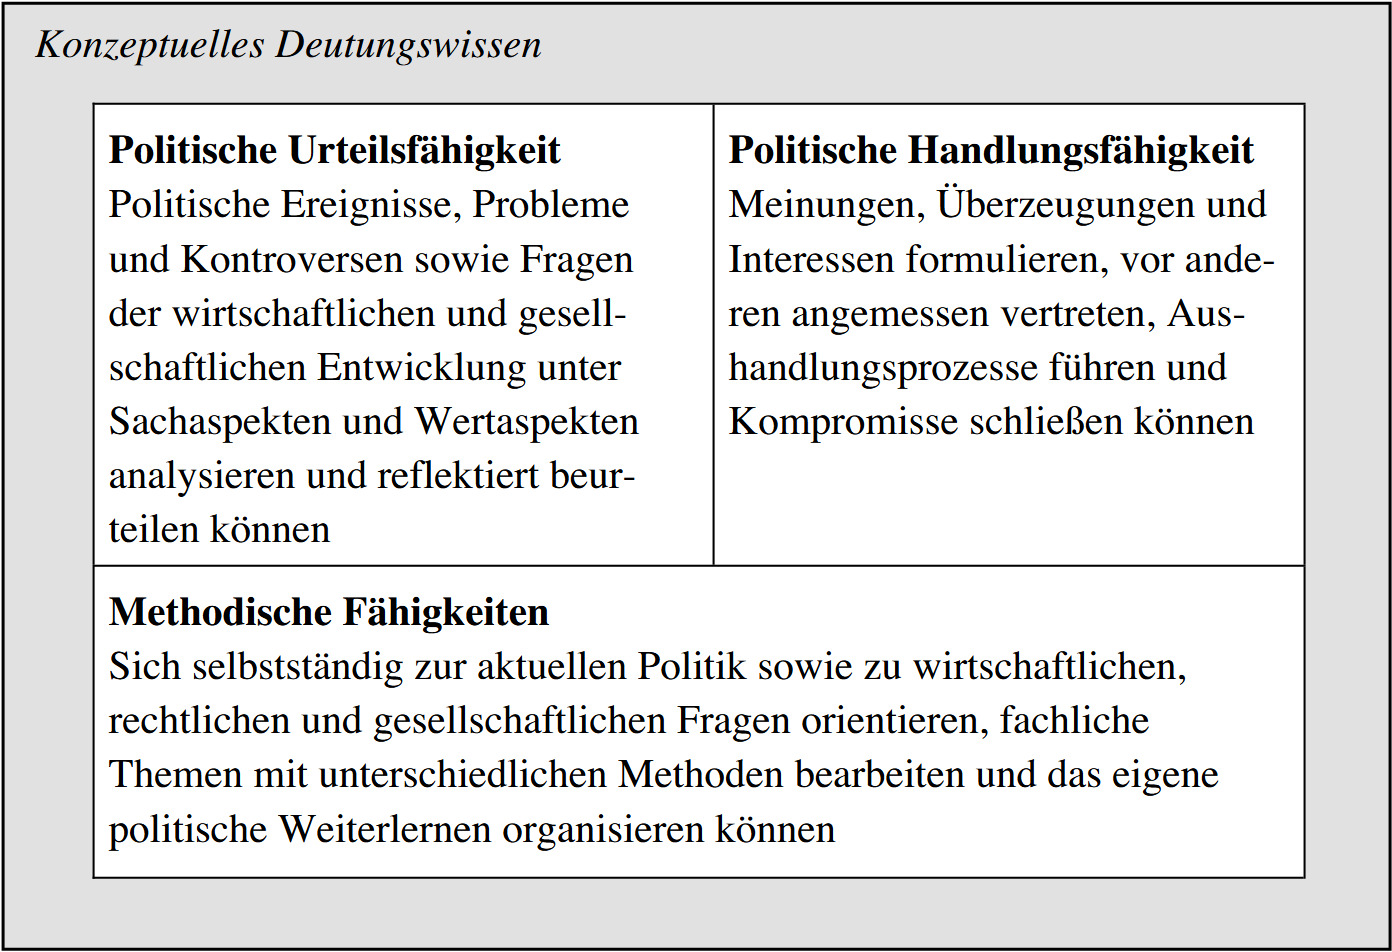
\includegraphics[width=1\linewidth]{gpje 2004 Kompetenzmodell S. 13.png}
    \caption{Kompetenzmodell der \gls{gpje} \autocite[übernommen nach][13]{gpje2004}. Genauso auch im Bildungsplan \autocite[10]{bplan} zu finden.}
    \label{gpjeKompetenzmodell}
\end{figure}

\textcite[106-107]{Gloe2020} skizzieren weiter, wie zu dieser Zeit auch 
\enquote{die eher sozialwissenschaftlich geprägte/n Vertreter[*innen] der Fachdidaktik Günter C. Behrmann, Tilman Grammes, Sibylle Reinhardt und Peter Hampe Kernkompetenzen} Kompetenzen der politischen Bildung als fünf \enquote{Demokratie-Kompetenzen} vorschlagen:
\begin{itemize}
    \item Wahrnehmung und Übernahme der Handlungsperspektiven Anderer, auch Dritter, zum Wechsel der eigenen Perspektive, zur Vermittlung des Eigeninteresses mit den Interessen Nah- und Fernstehender und dessen Ausweitung in Richtung auf allgemeinere Interessen (Perspektivenübernahme); 
    \item diskursiven Klärung konkurrierender und konfligierender Ideen und Interessen und zum Aushandeln von Konfliktregelungen und -lösungen (Konfliktfähigkeit); 
    \item problemorientierten Analyse struktureller Bedingungen und institutioneller Ordnungen sozialen, insbesondere politischen und wirtschaftlichen Handelns und zum Gebrauch sozialwissenschaftlicher Begriffe und Methoden (sozialwissenschaftliches Analysieren); 
    \item Einschätzung und Bewertung gesellschaftlicher Problemlagen, politischer Forderungen, Handlungschancen und -alternativen sowie zum reflektierten Gebrauch von Urteilskriterien (politische Urteilsfähigkeit); 
    \item Beteiligung an bürgerschaftlicher Selbstverwaltung, sozialen und politischen Initiativen, innerbetrieblicher und -organisatorischer Mitbestimmung, informellen und formalisierten Prozessen öffentlicher Meinungs- und Willensbildung (Partizipationsfähigkeit/demokratische Handlungskompetenz) 

    (\textcite[337 f.]{Behrmann.2004} zitiert nach \textcite[106-107]{Gloe2020})
\end{itemize}

\textcite{weißeno.2010} Ein weiteres Kompetenzmodell kam dann  mit dem \citetitle{weißeno.2010} von  auf.
 
\citeyear{weißeno.2010}


\begin{figure}[h]
    \centering
    \includegraphics[width=1\linewidth]{Weißeno et al. 2010 p.12.png}
    \caption{Kompetenzmodell nach \autocite[12]{weißeno.2010}}
    \label{2010kompMod}
\end{figure}



Artikulieren Argumentieren Verhandeln Entscheiden - APuZ 46–47/2012 \autocite[27]{Massing2012}



Kritik von Autorengruppe Fachdidaktik 2011 Quelle suchen




Dann abgewandeltes Modell \autocite[]{Detjen.2012}



Massing stellt diesen Zusammenhang wie ein beleidigter Frosch nicht her nicht her\autocite[23]{Massing.2022}



Autorengruppe Fachdidaktik:
Wolfgang Sander, Sibylle Reinhardt, Andreas Petrik, Dirk Lange, Peter Henkenborg, Reinhold Hedtke, Tilman Grammes, Anja Besand
\autocite[]{Sander.2016}
digggaaaaahhh wohin gehört der bums?\autocite[]{Sander.2016}



%%%%%%%%%%%%%%%%%%%%%%%%%%%%%%%%%%%%%%%  

%  Wolfgang Hilligen hatte in der schon erwähnten Untersuchung von 1955 Zur Auflösung der Fußnote[7] seine didaktischen Grundsätze bereits skizziert und damit zur Formulierung der Hessischen Richtlinien von 1957 beigetragen; seit diesem Jahr gibt es von ihm eines der bekanntesten Schulbücher („Sehen-Beurteilen-Handeln“) für den politischen Unterricht. Seine didaktische Konzeption entstand nicht aus einer vorgängigen wissenschaftlich-systematischen Überlegung, sondern umgekehrt aus den Schwierigkeiten der Unterrichtspraxis selbst, für deren Lösung er nach einer verallgemeinerungsfähigen, d. h. auch für andere Lehrer in gleicher Lage nützlichen Theorie suchte. Weil er diese im Laufe der Zeit immer wieder modifizierte und präzisierte, ist sein Wirken bis in die achtziger Jahre hinein eine wichtige Quelle für das Studium der Schwierigkeiten, die angesichts fortschreitender politischer und wissenschaftlicher Veränderungen mit einem solchen Vorhaben verbunden sind.  (Giesecke 1999, S. 15)
% Literaturverzeichnis
% Giesecke, Hermann (1999): Entstehung und Krise der Fachdidaktik Politik 1960-1976. In: Aus Politik und Zeitgeschichte (APuZ) (7-8), S. 13–23. Online verfügbar unter https://www.bpb.de/shop/zeitschriften/apuz/archiv/538800/apuz-7-8-1999/, zuletzt geprüft am 28.05.2025.
„Sehen-Beurteilen-Handeln“ auch schon in den 50er Jahren ein Ding, guck hier \autocite[15]{Giesecke.1999}

Fischer Prinzip \autocite[]{Grammes.2005}

ZITAT
Zum Verhandeln gehören neben argumentativen Strategien, die der konsensuellen Entscheidungsfindung dienen, auch Strategien, die durch den Einsatz von Machtpotenzialen, Konfliktfähigkeit, ökonomischen Ressourcen oder Tausch versuchen, Verhandlungsprozesse abzukürzen und zu hierarchisch autoritären oder hierarchisch majoritären Entscheidungen zu gelangen. Diese lassen sich im Unterricht zwar nicht erfahren, sollten aber gewusst werden. Entscheiden als Teil des realen partizipativen politischen Handelns lässt sich im Unterricht nur begrenzt fördern. Auch wenn Entscheiden durch kooperative oder handlungsorientierte Methoden geübt werden kann, bleibt es gegenüber der realen Politik unterkomplex. Allerdings lassen sich an konkreten politischen Fällen, Problemen, Konflikten oder Entscheidungsprozessen unterschiedliche Strategien und ihre Wirksamkeit analysieren, deren Ergebnisse den Lernenden dann als Fachwissen zur Verfügung stehen. (Massing 2012, S. 27)Literaturverzeichnis
Massing, Peter (2012): Die vier Dimensionen der Politikkompetenz. In: Aus Politik und Zeitgeschichte (APuZ) 62 (46-47), 23-28. Online verfügbar unter https://www.bpb.de/shop/zeitschriften/apuz/148228/politische-bildung/, zuletzt geprüft am 20.05.2025.

% bin bei gloe2020 s. 116 pdf118


ZITAT
Das Leitmotiv einer Pädagogik der Lernhilfe hat sicher den Vorteil einer pragmatischen Sicht auf den Lehrerberuf. Problematisch an dem Modell ist allerdings, dass es die Schule von den sozialen Problemen von Schülerinnen und Schülern in der heutigen Gesellschaft entkoppelt (Böhnisch/Schroer 2011). (Sander et al. 2016, S. 51)Literaturverzeichnis
Sander, Wolfgang; Reinhardt, Sibylle; Petrik, Andreas; Lange, Dirk; Henkenborg, Peter; Hedtke, Reinhold et al. (2016): Was ist gute politische Bildung? Leitfaden für den sozialwissenschaftlichen Unterricht. Schwalbach/Ts.: Wochenschau Verlag (Wochenschau Politik).
\autocite[]{Sander.2016}



Kompetenzen können kritisiert werden, es gibt Ähnlichkeiten. \enquote{Sie leisten die Verbindung zwischen den jeweiligen Bildungszielen der Fächer und den Aufgabenstellungen des Unterrichts (Detjen et al. 2012, S. 20)} \autocite[18]{Massing.2022}


Ähnlich vernichtend wie \textcite[][]{Roler2016} den Beutelsbacher Konsens auseinanderbastelt, ließe sich der nur bemüht als praxisnah zu empfindenden Debatte um Kompetenzen gegenüberstehen. Allerdings 



\subsection{Beutelsbacher Konsens} \label{bbk}% Beeinflussung durch Material.
Da insbesondere durch die Schulpflicht \autocite{BremSchulG} die schulische (politische) Bildung mit Zwang verbunden ist, liegt es nahe, dass versucht wird, diese durch Regeln, trotz des Zwanges, mit freiheitlichen, demokratischen Grundwerten zu vereinbaren. 

Ein wichtiges historisches Dokument im Rahmen derartiger Fragestellungen ist der \gls{bbk} \autocites[29]{Gesner2016}{Wehling1977}. So wichtig, dass auch über den deutschen Raum hinaus auf den \gls{bbk} Bezug genommen wird. So wurde jüngst im Rahmen der Aktionstage Politische Bildung vom 23. April bis 9. Mai 2024 in Österreich formuliert, dass der \gls{bbk} \enquote{[v]on internationaler Bedeutung [...] ist [...]. \autocite{bbkÖsterreich2023}}. Entsprechend leitet auch der Bremer Bildungsplan zentrale Kompetenzen aus dem \gls{bbk} ab und gibt ihn \enquote{im Wortlaut} wieder \autocite[11-12]{bplan}. 



\subsection{Bildungsplan für berufsbildende Schulen oder allgemeine politische Bildung mit Zielgruppenorientierung?}
% Politik an berufsbildenden Schulen in Bremen wird neben Deutsch als einziges Fach für alle Fachrichtungen berufsübergreifend unterrichtet. 
Daher findet sich strukturell wenig Unterscheidung zu dem Fach Politik an allgemeinbildenden Schulen.
Der Bremer Bildungsplan für Politik in der Berufsbildung ist mit der Veröffentlichung 2023 auch wesentlich aktueller als die Bildungspläne welche Politik beinhalten von 2006, 2008 und 2010 für die allgemeinbildenden Schulen in Bremen. 
Mit der Arbeitnehmerkammer Bremen wird sich außerdem auf einen lokalen Akteur bezogen, welcher voraussichtlich auch für einen Großteil der Bremer Schüler:innen an allgemeinbildenden Schulen relevant werden könnte. 
Zumal die politische Bildung an Berufsschulen sich explizit nicht auf den beruflichen Bereich beschränken soll, sondern gesamtgesellschaftliche Zusammenhänge zum Thema hat. Genau wie an allgemeinbildenden Schulen und bei politischer Bildung im Allgemeinen.


% Politische Bildung ist (oder sollte) in zahlreichen Lebensbereichen verortet (sein). Daher sei auf das Offensichtliche hingewiesen. Es handelt sich hier um Unterrichtsmaterial, welches für die staatlich institutionalisierte Bildung eingesetzt werden soll. 
% Dieses Bildungsmaterial soll jedoch mit einem anderen staatlichen Akteur herausgegeben werden. 


Wie werden Demokratiekompetenzen gefördert? Wird Wissen über Demokratiekompetenzen gefördert oder gar direkt demokratisches oder eben undemokratisches Handeln erprobt und reflektiert?



\subsection{Sozioökonomische Bildung, politische Bildung und interdisziplinäres Begriffs Wirrwarr} \label{polBildung}

Politische Bildung % im Kontext staatlicher Bildungsakteure 
ist im Schulkontext häufig nicht nur im Fach Politik, Sozial- oder Gemeinschaftskunde verortet, sondern auch häufig in Fächern mit Bezeichnungen, in denen \enquote{Politik} gleichbedeutend neben \enquote{Wirtschaft} genannt wird. 
So finden sich im Sachstandsbericht der Wissenschaftlichen Dienste des Deutschen Bundestags (\citeyear[5]{WD8.2016}) Fächerbezeichnungen wie \enquote{Politik / Gesellschaft / Wirtschaft} für Hamburg, \enquote{Politik und Wirtschaft}, \enquote{Politik-Wirtschaft} \& \enquote{Wirtschaft/Politik} in Hessen, Niedersachsen und Schleswig-Holstein oder \enquote{Gemeinschaftskunde / Rechtserziehung / Wirtschaft} für Sachsen. Damit ist in 5 von 16 Bundesländern politische Bildung schon in der Fächerbezeichnung an Wirtschaft gekoppelt \autocite[vgl. zu der tatsächlichen Zeit, die für politische Bildung im Unterricht an allgemeinbildenden Schulen zur Verfügung steht auch][14 \& 16]{Gokbudak2020}.

Materielle Bedingungen in der Sphäre des Politischen sind nicht von der Hand zu weisen. Die Beschäftigung mit materiellen Verhältnissen in der politischen Bildung respektive mit Wirtschaft ist also naturgegeben.
Als Forschungsfeld wird daher gerne auch von Sozioökonomischer Bildung gesprochen.
Insbesondere zu diesem Begriff lässt sich Forschung zu Unterrichtsmaterial und Einflussnahme externer Akteur*innen finden.


Die Bezeichnungen sowohl von Forschungsdisziplinen als auch von Schulfächern, versuchen dieser interdisziplinären Verknüpfung mal mehr, mal weniger gerecht zu werden.
Da die Trennschärfe solcher Begriffe Gefahr läuft, eine philosophische und linguistische Debatte über die Unzulänglichkeiten von Sprache zu eröffnen, wird in dieser Arbeit stets versucht, ein nach Ansicht des Autors möglichst passenden Begriff für den gerade gemeinten Gegenstand zu nutzen, welcher aber explizit nicht beansprucht, dass andere Begriffe aus leicht verändertem Blickwinkel nicht ebenso passend wären und lediglich eine notwendige Entscheidung darstellt. 

% Der Begriff Politik Wirtschaft ist dabei 


Gesellschaft und Kultur beeinflussen Wirtschaft.




\subsection{Arbeitnehmerkammer Bremen (ANK)}
Im Gesetz über die Arbeitnehmerkammer im Lande Bremen \autocite[]{ArbnkG} ist festgesetzt, dass nach der Beitragsordnung \autocite[]{ArbnkB} Beiträge nahezu aller Arbeitnehmenden\footnote{ 
Auf der Lohnabrechnung für einen Minijob taucht \gls{zb} kein Abzug für die \gls{ank} auf. Dies orientiert sich an der Geringfügigkeitsgrenze, welche für 2025 556€ beträgt \autocites{b.gering}{banz.gering}.
}
in Bremen zu erheben sind. Systemisch ähnlich zu Steuerzahlungen ist die Mitgliedschaft in der Kammer daher mit Zwangsbeiträgen verbunden. 

Im Gesetz zur \gls{ank} ist in \S2(1) \autocite[1]{ArbnkG} zu den Aufgaben der Kammer unter anderem formuliert: \enquote{Maßnahmen zur Förderung und Durchführung der beruflichen sowie der allgemeinen und politischen Weiterbildung der Kammerzugehörigen zu treffen}.

Da die \gls{ank}, wie der Name schon vermittelt, durchaus partikulare Interessen der Arbeitnehmer*innen vertritt, 


\subsection{Unterrichtsmaterial}
Der Begriff Unterrichtsmaterial soll in etwa synonym zur Definition auf der Website der \textcite{KMKMittel} für Lehr- und Lernmittel verwendet werden: 
Es gibt eine Lernmittelfreiheit \autocite[]{KMKMittel}.
Welches Unterrichtsmaterial am Ende auch in Kontakt mit den Schüler*innen kommt, liegt hauptsächlich in den Händen der Lehrer*innen.
Die Lehrkräfte selbst sind bei der Auswahl des Materials jedoch zahlreichen Zwängen ausgesetzt:
\begin{itemize}
    \item Zeitliche Zwänge: Der Tag hat nur 24 Stunden und Menschen sind Tiere mit zahlreichen Bedürfnissen. Diese zu erfüllen ist Voraussetzung für eine gute Arbeitsleistung, nimmt jedoch, genau wie Arbeit selbst, Zeit in Anspruch. 
    \item Finanzielle Zwänge: Schulen stehen begrenzte Budgets zur Verfügung, z.B. sind Schulbücher häufig nicht die \enquote{besten} und aktuellsten am Markt und Exkursionen müssen für alle bezahlbar sein. 
    \item Bereits am Markt existierendes Material ist entweder kostspielig und/oder unterliegt nur unzureichenden Qualitätskontrollen. Die Prüfung und Umgestaltung, um im Unterricht eingesetzt werden zu können, nimmt wiederum viel Zeit in Anspruch. 
\end{itemize}

Unterrichtsmaterial wird häufig aus dem Internet bezogen \autocite[82]{Neumann2015}. % zitiert nach \autocite[66]{Hedtke2016}




\subsection{\enquote{Wahrheit}, \enquote{Wahrhaftigkeit} und \enquote{Richtigkeit}} \label{wahr}

Für die Argumentation im Abschnitt der Medienkompetenz (\gls{abs} \ref{media}, \gls{S} \pageref{media}) ist eine Begriffsdefinition der drei Begriffe aus der Überschrift hilfreich. Da diverse Kompetenzmodelle der politischen Bildung auch die politische Handlungsfähigkeit als Ziel attestieren und zu dieser auch Meinungsbildung gehört -- ist es praktisch, dass diese Begriffe im Rahmen eines Kommentars zu dem Begriff Meinung dargestellt werden\footnote{Der folgende Abschnitt ist übernommen aus einer Hausarbeit von \textcite[4]{Klein2022}}:

In dem Essay \enquote{Bloße Meinung} beobachtet Frank \textcite[]{Nullmeier2019} kritisch, wie als Reaktion auf Desinformation eine absolute Wissenschaftlichkeit gefordert wird, welche die Meinung mit einem Anspruch auf Wahrheit \enquote{auf die Seite des zu Verwerfenden} \autocite{Nullmeier2019} stellt.  Weiterhin bezieht Nullmeier sich auf drei Begriffe für Wahrheit:
\begin{enumerate}
    \item Wahrheit: Als Wahrheit empirischer Aussagen.
    \item Wahrhaftigkeit: Als Begriff um mit Unwahrhaftigkeit die Lüge kennzeichnen zu können - In der Abgrenzung zu Unwissen oder sich als falsch erweisenden empirischen Wahrheit. In der Lüge ist die Wahrheit enthalten, sie wird nur nicht gesagt. 
    \item Richtigkeit: Als Begriff, um eine Wahrheit für normative Aussagen zu haben, die sich aus \enquote{eine[r] partiell wahrheitsanaloge[n] Logik der Argumentation mit der Annahme einer aus richtig und falsch bestehenden Binarität und einer potenziell allein richtigen Aussage [er]geben} \autocite{Nullmeier2019}.
\end{enumerate}

Er führt aus, dass Meinung in demokratischen, politischen Entscheidungsprozessen von einer immanenten Wichtigkeit ist. Entsprechend wichtig sollte die Meinung daher auch im Politikunterricht sein.




\subsection{Medienkompetenz und die unbedingte Verknüpfung zu \enquote{Wahrheit}}\label{media} 
Medienkompetenz sollte in allen Fächern der Schule grundsätzlich, aber aufgrund der großen Schnittmenge insbesondere im Politikunterricht mitgedacht und mitgemacht werden. 
Noch konkreter argumentiert: Medienkompetenz ist lediglich ein bestimmte Bereiche betonender Begriff für integrale Lerngegenstände von politischer Bildung. Diese Lerngegenstände ergeben sich aus der Zielsetzung der geforderten Kompetenzen. Eine konkrete und praktische Umsetzung von Medienkompetenz kann dabei in Quellenarbeit und Zitation gesehen werden.
 
\subsubsection{Die Zerteilung der Welt durch Worte}
Daher nun ein kleiner philosophischer Ausbruch in die Verknüpftheit von Wissen und Sprache: Auch in dem Entstehungszeitraum der vorliegenden Arbeit sind \enquote{Wahrheit}, \enquote{Wahrhaftigkeit} und \enquote{Richtigkeit} nicht nur in der Kommunikation grundsätzlich, sondern insbesondere auch im Politischen eine zentrale Debatte. 
Im Zeitalter von Desinformation, \enquote{framing}, Populismus und Propaganda ist für die Erziehung zu mündige(re)n Menschen die Auseinandersetzung mit der Produktion von Wissen und \enquote{Wahrheit} unerlässlich. Die im vorigen Satz aufgezählten Begriffe enthalten immer eine Form \enquote{Unwahrhaftigkeit} oder das (teils bewusste) Auslassen von \enquote{Wahrheit}. Um die verschiedenen Formen und Unterschiede des Irrens und der Lüge durchdringen zu können, ist entsprechend ein Anschneiden dieses Themenkomplexes unerlässlich.  

Über das bloße, eher oberflächliche, Verstehen von Inhalt selbst hinausgehend, ist ein wesentlicher Bestandteil von Medienkompetenz, den Inhalt bewerten zu können. In diesem Zusammenhang soll bewerten bedeuten, den Inhalt mit anderen Dingen zu verknüpfen. Denn da Wissen (oder \enquote{Wahrheit}) grundsätzlich in Beziehung von Subjekten zur Welt und Beziehung untereinander erschaffen wird, ist es geradezu unabdingbarer Bestandteil eines verstehenden Wissenserwerbs, das Wissen auch mit dem Kontext, in welchem es entstanden ist, zu verknüpfen. Das Verknüpfen von Wissen ist dementsprechend auch Voraussetzung für ein tiefergehendes Verstehen. 

Die Diskussion, inwiefern Wissen auf Logik basierend auch mit wenig Beziehung zu anderen Subjekten und der dinglichen Welt \enquote{erschaffen} oder \enquote{erkannt} werden kann, soll an dieser Stelle ausgeklammert werden. Denn pragmatisch gesehen ist jede Form von Information in der physischen Welt mindestens als Energiezustand verankert. Menschen lernen das Denken insbesondere an ihren über die Sinnesorgane vermittelten Erfahrungen mit der dinglichen Welt, was dann erst mit der Zeit höhere Abstraktionsebenen (Symbole, Sprache, Wittgenstein \gls{etc} gib' ihm) ermöglicht. Und auch noch so stark abstrahierte Informationen sind eben immer noch mindestens irgendwie messbar in der physischen Welt verankert. Sei es eine Schallwelle des gesprochenen Wortes, eine neuronale Verbindung im Gehirn, Spannung oder Magneten in einem Computer, Symbole auf Papier oder spezifisch angeordnete Basentriplets einer messengerRNA auf dem Weg, ein Protein synthetisieren zu lassen. 

Ein eingängiges Beispiel für die unbedingte Verknüpftheit von Wissen lässt sich am Wort \enquote{Baum} darstellen. Erstens muss -- um dem Wort eine über den Zufall hinausgehende Bedeutung zu verleihen -- mindestens irgendein Subjekt das Wort tatsächlich mit einem Konzept von Baum verknüpfen. Wenn Sprache ihre Funktion der Kommunikation -- unter der wir sie kennen -- erfüllen soll, am besten mehrere Subjekte.
Ferner könnte ein Baum nicht existieren ohne Wasser, die Energie der Sonne, Jahrmillionen an Evolution, Erde \gls{etc} Sprache zerlegt eine zwangsläufig verknüpfte Welt immer in Bestandteile. 
Wer das Konzept (also das Wort und das Wissen, welches es bezeichnet) \enquote{Baum} verstehen möchte, weiß in irgendeiner Form auch Teile dieses zwangsläufigen verknüpften Wissens. Denn um das Wort \enquote{Baum} gebrauchen zu können, wird der Baum von der Sonne und aus der Erde herausgetrennt. Wenn das nicht so wäre, gäbe es keine Worte. Weil konsequent zu Ende gedacht immer nur ALLES ausgedrückt werden könnte, da über genügend Umwege alles miteinander verknüpft ist. 

\vspace{12pt}
\hrule
\vspace{12pt}

back to it


\subsubsection{Quellen}

An diese Quellendarstellungen muss sich im Sinne der didaktischen Reduktion jetzt nicht sklavisch gehalten werden.
Als polemisches Beispiel: Im Mathematikunterricht in der Elementarstufe bedarf es womöglich zu viel mental load, um auf die Verschriftlichungen von Adam Ries Bezug zu nehmen. Aber vom Grundsatz her ist es durchaus angebracht, so viel Quellenmaterial wie möglich, so präzise wie möglich auch im Unterrichtsmaterial selbst mitanzugeben. Alleine um mit gutem Beispiel voranzugehen. 
% Diggah, mach halt immer ehrenloses Scheißquellengeballer, anstatt Infos gehaltloser rauszuballern als gmx.de newsflash. Medienkompetenz ist Sack, die Medienlandschaft und Lehrmaterial sind aber auch häufig genug beschämendes Negativbeispiel. Jeder Scheiß Porno hat mit seinen blöden Wasserzeichen mehr Qualität in der Nachverfolgbarkeit der Urheberschaft. Man


Eine gute Vorbildfunktion ist essentielle Voraussetzung für verschiedene Formen des Lernens, wie es theoretisiert wird.
Egal, ob es sich um das Beobachtungslernen \autocite[73ff.]{Kiesel2012} welches maßgeblich von Albert Bandura definiert wurde, handelt, oder ob im Rahmen des (zwar umstrittenen) impliziten Lernens \autocite[83ff.]{Kiesel2012} stattfindet. Ohne ein auch positiv-Beispiel zu haben, wird das Erlernen von der Relevanz und der methodischen Durchführungsmöglichkeiten einer guten Quellenarbeit erschwert. Aus dem Grunde ist der Bildungsbereich von Beginn an gut beraten, stets gute Beispiele für die Quellenarbeit darzustellen. 


Darüber hinaus Einstellung \autocite[130]{Kiesel2012}



\subsection{Zielgruppe}
Gutes Unterrichtsmaterial ist nicht per se gut, sondern es ist lediglich abhängig von den Rezipient*innen gut. Eine womöglich gut vorbereitete Lerneinheit zu Polynomdivision für Studierende in Höherer Mathematik ist in einer Elementarstufe, die gerade überhaupt dividieren lernt, sicherlich nicht mehr gut. Gutes Unterrichtsmaterial ist also in erster Linie für die intendierte Zielgruppe zu untersuchen. Jede Lerngruppe ist individuell, dennoch lässt sich allein durch das Alter, den Lernort und -- zum Teil  mit dem Ort einhergehend -- die Sprache und viele weitere Faktoren, die Lerngruppe bereits stark abgrenzen. Genau das passiert auch bei einem Englischbuch, welches für Unterricht auf Deutsch in der 5./6. Klasse in Baden-Württemberg veröffentlicht ist. 

Es ist also angezeigt, die Zielgruppe des Unterrichts möglichst klar abzugrenzen, wenn untersucht werden soll, ob Material \enquote{gut} ist. 


Wenn es dann genauer an die Planung von konkretem Unterricht geht, sind insbesondere die Lehrpersonen gefordert, um auf den Wissensstand und bestehende Schüler*innen-Vorstellungen eingehen zu können. Nach dem Modell der didaktischen Rekonstruktion sollen Lerninhalte besser und nachhaltiger vermittelt werden, wenn dies geschieht \autocite[404-406]{Reinfried2009}.

Dadurch, dass das Material mit Fokus auf duale Studiengänge berufsbildende Schulen erstellt ist, unterscheidet sich die Zielgruppe von der an allgemeinbildenden Schulen in dem wesentlichen Punkt, dass gerade der Lebensweltbezug für Arbeitsthemen durch die eigenen Arbeitserfahrungen im Betrieb deutlich weniger theoretisch ist, als wenn an einer Oberschule zum Beispiel über Arbeitsschutz gesprochen wird. 

\enquote{Fremdzuschreibungen und defizitorientierte Ansprachen von Personengruppen sind deshalb problematisch, weil sie die in unserer Gesellschaft ungleich verteilten Zugänge zu u.a. Bildung und Chancen mitunter eher reproduzieren als sie – wie von einer inklusiven politischen Bildung} \autocite[]{Beckmann2022}
Dennoch ist es wichtig, die Zielgruppe zu kennen und darauf einzugehen.



2024-12-11
Wie wird die Zielgruppe angesprochen?
Wird eine heterogene Zielgruppe angesprochen?
Bla über Defizitorientierung
% https://profession-politischebildung.de/grundlagen/grundbegriffe/defizitorientierung/#:~:text=Defizitorientierung%20meint%20die%20Fokussierung%20auf,Bildungsangeboten%20sowie%20im%20p%C3%A4dagogischen%20Handeln.
% die website zitiert z.B: bei Citavi Holzer 2010

\subsubsection{Schüler*innenvorstellungen}
Nach dem Modell der didaktischen Rekonstruktion \autocite[]{Reinfried2009} ist die Inbezugnahme von Schüler*innenvorstellungen ein zentrales Element für besseren Unterricht.
Es soll also untersucht werden, an welchen Stellen das Material Schüler*innenvorstellungen aufgreift oder immerhin Raum dafür lässt. 

\subsection{Was sagt die Wissenschaft zu politischer Bildung an (Berufs)schulen?}
Anja Besand

Reinhold Hedtke (den habe ich schon)

Bettina Zurstrassen (Herausgeberin Sammelband von der bpb) 

Christine Engartner



Die \gls{ank} als Gegenspieler zu wirtschaftsnahem Material? Engartner 2023:7

\subsection{Ökonomische versus politische Sozialisation?}
In der Forschung zu politischer Bildung in staatlichen Institutionen wird seit geraumer Zeit verhandelt, wie die Einflussnahme externer Akteure zu bewerten sei. Reinhold Hedtke 

Autor*innen, welche einen bildungstheoretischen und/oder einen politikwissenschaftlichen Hintergrund aufweisen, lesen sich insofern ähnlich, als dass ihnen gemein ist eine gute politische Bildung interdisziplinär zu gestalten. Insbesondere für den berufsbildenden Bereich lässt sich feststellen, dass Forderungen erwachsen, die \enquote{betriebswirtschaftlichen Verwertungslogiken}

dritte Säule \autocite[]{kerschensteiner1966}
% Diggah, wie soll ich Forschungsüberblick geben, wenn alleine Reinhold Hedtke gefühlt gut 200 Veröffentlichungen zur gleichen schmackhaften Soße hat?


\subsection{Mehr Platz für Emotionalität}
Gutes Unterrichtsmaterial gibt die Beziehungsebene zwischen Lehrer*innen und Schüler*innen nicht vor, aber sorgt im Idealfall durch gute Strukturierung und guten Umgang mit den bestehenden Ressourcen dafür, dass die Beziehungsebene mehr Platz bekommen kann.

Gleichzeitig sind Emotionen integraler Bestandteil des Politischen \autocite{Heidenreich.2012a} und sind daher nicht in einem veralteten Dualismus (der Rationalität unverbunden und moralisch unterlegen) aus dem Unterricht zu verbannen. % Auch wenn in dieser Hinsicht noch reichlich Nachholbedarf besteht. 

Dass Emotionen gerade in Zusammenhang mit Politik bisweilen einen faden Beigeschmack haben, trägt Hendrik Schröder (\citeyear[4-5]{Schroder.2020}) 



\subsection{Veröffentlichungsreichweite, Auffindbarkeit, Preis, Einsetzungsreichweite} \label{öffi}

Es darf davon geträumt werden, Unterrichtsmaterial, welches durch öffentliche oder fast öffentliche Gelder finanziert wurde, auch der Öffentlichkeit zugänglich ist.

\subsection{Forschungsfrage}
Wie lässt sich das Unterrichtsmaterial der Arbeitnehmerkammer Bremen bewerten?

Wie und nach welchen Maßstäben lässt sich das Unterrichtsmaterial der Arbeitnehmerkammer Bremen bewerten?

\section{Analysemaßstab}
Analyse

Im Sachunterricht in der Elementarstufe wird kritisiert, wenn der Unterricht wenig mit der eigentlichen Sache zu tun hat \autocite[2-4]{Scholz2004}. Im Politikunterricht ist das Anschauen jedoch weniger auf Dinge bezogen. Analog dazu lässt sich jedoch die bereits im \gls{bbk} geforderte Handlungskompetenz sehen. Spannend ist es also zu untersuchen, inwiefern durch das Material politisches Handeln beobachtbar oder gar an der eigenen Gruppe erlebbar wird.


\subsection{Fragen an das Material} % Nach welchen Maßstäben Unterrichtsmaterial analysieren?
Ein eher offen formulierter Bildungsplan ist kein Zufall. % Aus ähnlichen Gründen, die einen offen formulierten Bildungsplan nahelegen,
Daher wäre es kontraindiziert, Unterrichtsmaterial nach starren Vorgaben zu bewerten.
Dennoch soll eingegrenzt werden, nach welchen Maßstäben Unterrichtsmaterial bewertet werden könnte. Offen bedeutet nicht beliebig.

Die erste Anlaufstelle dafür ist der Bildungsplan selbst. In Anlehnung an die Gliederung des Bildungsplans kann das Unterrichtsmaterial anhand folgender Punkte untersucht werden:
\begin{itemize}
    \item Kompetenzen jeweils der beruflichen \& politischen Bildung
    \item Lebensweltorientierungen % Modell der didaktischen Rekonstruktion
    \begin{itemize}
        \item Arbeits-,  Berufs- und Lebensweltorientierungen
        \item Problem-, und Wissenschaftsorientierungen
        \item Zukunfts-, Gegenwarts- und Vergangenheitsorientierungen
    \end{itemize}
    \item Methodische Grundsätze
    \item Und anhand folgender sieben politischen Handlungsfelder:
    \begin{itemize}
        \item Demokratie 
        \item Gesellschaft 
        \item Arbeitsleben
        \item Öffentlichkeit im digitalen Zeitalter
        \item Wirtschaftspolitik
        \item Globale Zusammenhänge 
        \item Nachhaltigkeit 
    \end{itemize}
\end{itemize}


Im Bildungsplan sind die drei wichtigsten Kompetenzen in Anlehnung an den \gls{bbk} formuliert. 

\begin{itemize}
    \item Politische Urteilsfähigkeit
    \item Politische Handlungsfähigkeit
    \item Methodische Fähigkeiten 
\end{itemize}

Daher soll im nächsten Schritt analysiert werden, inwieweit das Unterrichtsmaterial diese Kompetenzen fördert. 

% Maßgeblich dafür können Vergleiche zu Bewertungskriterien sein, die bereits von anderen genutzt worden sind.
% Auch maßgeblich soll sein, inwiefern schon das Unterrichtsmaterial in Bezug auf den Bildungsplan und dessen, unter Anderem aus dem \gls{bbk} abgeleiteten, Kriterien vereinbar scheint. 


Fragen, die darüber hinaus und ergänzend an das Material gestellt werden sollen, sind:
\begin{itemize}
    \item Welche Kompetenzen werden an welcher Stelle gefördert?
    \item Wie und durch welche Operationalisierung werden die Kompetenzen gefördert?
    \item Wie werden Schüler*innenvorstellungen berücksichtigt? % zB diametral entgegen falscher Vorstellungen oder auf richtige Vorstellungen aufbauend? Außerdem: Stichwort: Reifizierung \autocite[]{Reinfried2009}
    Siehe auch die reflexiven Fragen für das Modell der didaktischen Rekonstruktion bei \textcite[411-412]{Reinfried2009}.
    \item An welchen Stellen soll induktiv, an welchen deduktiv vorgegangen werden?
    \item Ist das im Modell der Didaktischen Rekonstruktion sinnvoll? \autocite[]{Reinfried2009} Sollte im Sinne des Konstruktivismus besonders induktives Vorgehen seitens der SuS antizipiert werden?
    \item Wie wird Schüler*innenaktivität erzeugt? % Für Konstruktivismus wichtig
    \item Wird bestehendes Material benutzt und analysiert oder wird auch eigene Produktion angeregt?
    \item Wie ist die Ergebnissicherung eingebunden?
    \item Welche Handlungsfelder werden angesprochen?
    \item Inwieweit bietet ist das Material auf die Lebensrealität und realistische Partizipationsmöglichkeiten ausgerichtet?
    \item Inwieweit impliziert das Material politisches Handeln, welches bestehende Systeme in Frage stellt? Ist das noch vertretbar (im Konkreten: mit dem \gls{bbk} vereinbar)? Ist im Gegenzug ein Weglassen solcher Perspektiven vertretbar (im Konkreten: mit dem \gls{bbk} vereinbar)?
    \item Welche Medien werden eingesetzt? Wie ist die Wahl der Medien begründet?
    \item Medienkompetenz % siehe Demokratie ANK Dinger Kommentare für die Quellen M! und M2 letzte Seite
    \item Inklusion
    \item Digitalisierung (Methodenkompetenz. Sinnvoll eingesetzt?)
    \item Was wird vom Material an Möglichkeiten der Binnendifferenzierung geboten?
    \item Wo findet eine Binnendifferenzierung statt; sowohl im Inhalt als auch den Methoden? Ist die Wahl der Methoden aus der Didaktik zu begründen? Welche alternative Methoden wären möglich gewesen? Werden unterschiedliche Methoden für unterschiedliche Lerngruppen Angeboten?
    \item Handhabbarkeit, Anwendbarkeit, praktisches, pragmatisch. Handwerkliche Betrachtung
    \item Umfang, Zeitvorgaben, zur Verfügung Stellung realistisch?
    \item Unwahrscheinlich: Aber, ist das Material Alterdgruppen geeignet oder gar übergriffig?
    \item Welche Beeinflussungen sind zu erkennen? Lassen sich diese legitimieren?
\end{itemize}
Darüber hinaus soll untersucht werden, inwieweit sich Intentionen der Arbeitnehmerkammer Bremen im Material finden lassen und ob die Beeinflussungen des Akteurs sich in einem Rahmen bewegen, welcher der Intention des \gls{bbk} nicht entgegensteht. \#Kontroversitätsgebot 


\subsection{Bildungsplan als Analysemaßstab}
Der Bildungsplan \autocite{bplan} in Politik für duale Studiengänge im Land Bremen...

Wie zu Kapitelanfang angedeutet ist der Bildungsplan vergleichsweise offen formuliert, ohne detaillierte Vorgaben zu machen. Angesichts der überbordenden Themenauswahl und interdisziplinären Verstrickung eines Faches wie Politik eine konsequente Entscheidung, die im Bildungsplan selbst argumentativ legitimiert wird \autocite[diggah, welche Seite habe ich das gelesen]{bplan}. Reinhold \textcite[17-18]{Hedtke2016} kritisiert für den Wirtschaftsunterricht den fehlenden Bezug auf die Fachwissenschaften sowie auch eine fehlende Berücksichtigung der zahlreichen Interdependenzen zu benachbarten Fachwissenschaften. 


\subsection{Poltische Bildung in der Fachliteratur -- Ein Auszug}
Im Bremer Schulsystem werden in der Mittelstufe klassische Schulfächer wie Chemie, Physik und Biologie gemeinsam im Fach \gls{nw} \autocite{vogel2010nw} oder im sozialwissenschaftlichen Bereich wurden Geschichte, Politik und Geographie zu meiner Zeit an der Gesamtschule als \gls{wuk} \autocite{vogel2006gs} oder heutzutage an Oberschulen als \gls{gp} \autocite{vogel2010gp} unterrichtet.
% GEHT DIE ICH FORM??
->
Autor:innnen haben auch keinen Bock mehr auf monodisziplinär. 

Die \gls{bpb} hat den Sammelband veröffentlicht.
\subsection{Quellenangaben}
\begin{itemize}
    \item Wie lässt sich die Qualität der Quellen bewerten?
    \item Wie wird auf Medienkompetenz eingegangen?
 \end{itemize}




\section{Analyse}
Obgleich im Bildungsplan explizit formuliert ist, dass durch inhaltliche Offenheit \enquote{der Einsicht entsprochen [wird], dass eine konsensfähige Festlegung relevanter, zeitloser Inhalte weder fachwissenschaftlich noch fachdidaktisch begründbar ist} \autocite[15]{bplan}, wird verlangt, vier der sieben \enquote{politischen Handlungsfelder}, darunter \enquote{Demokratie}, zu bearbeiten. 

Das Material der \gls{ank} ist den im Bildungsplan vorgegebenen \enquote{politischen Handlungsfeldern} \autocite[15]{bplan} zugeordnet und erleichtert durch diese Vermeidung unnötiger Kompliziertheit eine Zuordnung und Einbettung in eine den Bildungsvorgaben entsprechende Grobplanung des Unterrichts.


\subsection{Demokratie}
Für den Bereich Demokratie sind zwei Themen angeboten:
\begin{enumerate}
    \item Demokratie A: \enquote{Föderalismus und Arbeitsschutz – Welche Chancen und Risiken bringt das Mehrebenensystem der BRD für die Sicherheit und Gesundheit am Arbeitsplatz mit sich?}
    \item Demokratie B: \enquote{Wahlen – von welchem Teil des Volkes geht eigentlich die Staatsgewalt aus?}
\end{enumerate}
Für beide Bereiche sind je drei Karten mit jeweils ausdifferenzierten Leitfragen vorhanden. Die drei Karten sind in der Struktur
\enquote{Einstieg},
\enquote{Erarbeitung} und
\enquote{Auswertung/Übertrag} 
bezeichnet. 


\subsubsection{Demokratie A - \enquote{Föderalismus und Arbeitsschutz – Welche Chancen und Risiken bringt das Mehrebenensystem der BRD für die Sicherheit und Gesundheit am Arbeitsplatz mit sich?}}
Am Beispiel des Themenbereiches \enquote{Demokratie A} (A1 bis A3) wird als Kompetenzbereich 
\blockquote{Die Schüler:innen sind in der Lage das Wesen der Demokratie, die Strukturen und Organisationen des politischen Systems sowie die Mechanismen politischer Willensbildung einzuordnen und zu beurteilen.}
angegeben. Diese Formulierung ist direkt aus dem Bildungsplan übernommen \autocite[][16]{bplan}.

Die Kompetenzen in Kompetenzbereiche einzuordnen, ist sicherlich sinnvoll, um einen Überblick zu haben, innerhalb welches Kompetenzbereiches exemplarisch gefördert wird und wo im Bildungsplan man bereits geübt hat und welche anderen Kompetenzen daher in Zukunft womöglich eher Aufmerksamkeit bedarfen. 
Denn wie stets ist es ausgeschlossen, nicht exemplarisch zu lernen. 

Da für eine einzelne Unterrichtseinheit jedoch kaum in Anspruch genommen werden kann, einen Kompetenzbereich hinreichend -- auch exemplarisch -- abzudecken, wäre es sinnvoll, noch konkreter anzugeben, welche exemplarischen Kompetenzen erworben werden.
In dem Fall der Materialkarten geschieht dies nicht über eine konkretere Ausdifferenzierung der Kompetenzen, sondern über die \enquote{Leitfrage}, das \enquote{Thema} und die \enquote{Keywords}. 

Unter den drei Karten für \enquote{Demokratie A} grenzt das Thema: \enquote{Föderalismus und Arbeitsschutz – Welche Chancen und Risken bringt das Mehrebenensystem der BRD für die Sicherheit und Gesundheit am Arbeitsplatz mit sich?} konkreter ein, was durch das folgende Material und die Aufgaben an Kompetenzen vermittelt werden soll. 
Die Leitfragen
\begin{enumerate}
    \item Demokratie A1: \enquote{Welche Erfahrungen mit Arbeitsschutz habt ihr bisher gemacht?}
    \item Demokratie A2: \enquote{Wer kümmert sich um den Arbeitsschutz?}
    \item Demokratie A3 \enquote{Pro und Contra Föderalismus oder warum ist das Teilen von Macht ein Strukturprinzip demokratischer Herrschaft?}
\end{enumerate}
teilen das Thema dabei in die drei Karten auf.


\subsubsection{Demokratie B - \enquote{Wahlen – von welchem Teil des Volkes geht eigentlich die Staatsgewalt aus?}}
Der am Bildungsplan orientierte Kompetenzbereich für den zweiten Lehrvorschlag unter dem Thema: \enquote{Wahlen – von welchem Teil des Volkes geht eigentlich die Staatsgewalt aus?}, lautet: \enquote{Die Schüler:innen sind in der Lage unterschiedliche demokratische Entscheidungsverfahren zu reflektieren und zu beurteilen.} \autocite[][16]{bplan}.


Leitfragen
\begin{enumerate}
    \item \enquote{Was denken eure Mitschüler:innen über das Thema Wahlen?}
    \item \enquote{Wer geht eigentlich wählen und warum ist das ein Problem?}
    \item \enquote{Warum wird in einer Demokratie gewählt?}
\end{enumerate}



\subsection{Arbeitsleben}
\enquote{Arbeitsleben A} 
Thema
\enquote{Arm trotz Arbeit – ist das gerecht?}


Leitfrage
\enquote{Was ist Einkommensarmut und wie kann sie erklärt werden? Welche Leistungen kann ich in Bremen beantragen, wenn ich von Einkommensarmut betroffen bin?}

Kompetenzbereich
\enquote{Die Schüler:innen sind in der Lage berufliche und gesellschaftliche Lebenssituationen vor dem Hintergrund der sich verändernden wirtschaftlichen und politischen Rahmenbedingungen zu erkennen, um adäquate individuelle Entscheidungen treffen zu können.}


Thema
\enquote{Wieviel verdienen  Arbeitnehmer:innen in Bremen und welche (politischen und wirtschaftlichen) Maßnahmen würde die Situation am Arbeitsmarkt verbessern?}


\enquote{Arbeitsleben B}
Thema
\enquote{Entgrenzte Arbeit – Haben wir bald nie wieder Feierabend?}

Leitfrage
\enquote{Welche gesetzlichen Grundlagen regulieren die Arbeitszeiten und wie kann ich mich vor entgrenzter Arbeit schützen?}


Leitfrage
\enquote{Welche gesetzlichen Grundlagen regulieren die Arbeitszeiten und wie kann ich mich vor entgrenzter Arbeit schützen?}




Kompetenzbereich
\enquote{Die Schüler:innen sind in der Lage, die derzeitigen Arbeitswelten mitsamt ihren Institutionen, Kulturen und Praktiken als historisch gewachsen beschreiben und als politisch veränderbar herauszuarbeiten.}

Thema
\enquote{Mitbestimmen oder nur dabei sein?}

Leitfrage
\enquote{Welche Aufgaben haben Gewerkschaften und wie ist der Interessenausgleich von Arbeitnehmer:innen und Arbeitgeber:innen (gesetzlich) organisiert?}


Leitfrage
\enquote{Politik meets Betrieb: Wie kann betriebliche Mitbestimmung die Demokratie stärken?}





\subsection{Wirtschaftspolitik} % ansonsten wohl Gesellschaft





\subsection{Den Themenfeldern gemeinsame Beobachtungen}

\subsubsection{Erwartungshorizont}
Ein Erwartungshorizont ist bei dem Material nicht mitgeliefert.
Ein Erwartungshorizont ist naturgemäß an die Zielgruppe anzupassen und im besten Falle binnendifferenziert, da davon auszugehen ist, dass jede Zielgruppe heterogen ist. Allerdings gilt das an jeder Stelle der Unterrichtsvorbereitung und des Unterrichtsmaterials. 
Ein exemplarischer Erwartungshorizont oder gar einer -- welcher verschiedene Abstufungen, von einem Minimum, um dem Kompetenzbereich gerecht zu werden, bis hin zu einem Ausblick, wo das eingegrenzte Thema überschritten wird, aber wo man weiter lernen könnte -- wäre eine hilfreiche Ergänzung, um die Vorbereitung der Lehrkräfte zu erleichtern. 

\subsubsection{Arbeitsblatt-Charakter}
Letzten Endes bleibt das institutionalisierte Lernen Arbeit für alle Beteiligten. Dennoch sollte hinsichtlich der hier untersuchten Unterrichtsvorschläge nicht unerwähnt bleiben, dass auch diese es selten schaffen, aus dem in der Überschrift erwähnten Arbeitsblatt-Charakter auszubrechen. Abwechslung der Methoden und zwischen Lesen, Schreiben und Sprechen, Wechsel zwischen Einzel-, Partner*innen- und Gruppenarbeit sowie Methoden im Plenum sind vorhanden und stellen damit eine solide Grundlage bereit. Der Ausbruch, um durch Ungewöhnliches Aufmerksamkeit oder Nachhaltigkeit des Lernens zu erzeugen, wird hingegen nicht gewagt. 
Auch das Training der \enquote{politischen Handlungsfähigkeit} bleibt auf dem für Schule nicht untypischen Niveau des entfremdeten Lernens. 

Der Anspruch der Unterrichtsvorschläge ist allerdings auch kein revolutionärer. Ohnehin ist es eine andere Diskussion, inwieweit die Schule als staatliche und stark bürokratisierte Institution bisweilen im Widerspruch zum freien Denken steht, welches immer wieder auch Bestandteil der Dinge ist, die sich in ihren Zielsetzungen lesen lassen. 

\enquote{Arbeitsleben B1} Debatte

\enquote{Stellt Euch folgendes Situation vor.} \enquote{Arbeitsleben B2}

\enquote{Welche politischen Rahmenbedingungen müssten geschaffen werden, um den Vorschlag umzusetzen?} \enquote{Arbeitsleben B3}

\subsection{Vorbildfunktion -- Beobachtungslernen}


\enquote{Arbeitsleben c} Martina Zandonella 
\enquote{Ja. Diese Menschen haben die Erfahrung gemacht: Für mich zahlt es sich nicht aus, meine Stimme abzugeben.}
Wahlbeteiligung vgl. \enquote{Demokratie}

\footnote{Lernende sind nicht dumm. Wenn in der Schule demokratische Übungen immer das bleiben: Übungen. Lernen sie, dass ihr politisches Handeln keine Auswirkungen hat. Das ist gefährlich.}

performative Mitbestimmung
Schule restriktive Institution

\autocite[][]{Elsasser.2017}




\subsection{Subjektive Einschätzung}
Gleichwohl das wissenschaftliche Arbeiten nach Objektivität streben sollte und sich diverser Kulturtechniken bedient, um diesem Ideal nahe zu kommen, ist eine subjektive Einflussnahme der Forschenden kaum auszuschließen. Aus diesem Grunde soll im Anschluss an % wirklich nach?
die kriteriengeleitete Analyse noch der subjektive Eindruck des Autors dargestellt werden. 

\subsection{Reflexion}
Die Frage nach der eigenen Produktionstätigkeit der \gls{sus} ist in Bezug auf die geforderte politische Handlungsfähigkeit interessant. Strukturell bleibt auch eine gut ausgebildete Analysefähigkeit auf einer Beobachtungsebene. Das ist für politische Handlungsfähigkeit zweifelsohne wichtig. Spannend ist jedoch, wie im Rahmen von Schulunterricht tatsächliche Erfahrungen von Gestaltung verwirklicht werden können. Die demokratische Legitimation ist am höchsten, wenn möglichst viele Menschen entweder tatsächlich an den Entscheidungen beteiligt waren oder zumindest eine hohe Identifikation mit den Entscheidungen aufweisen, auf welche sich geeinigt wurde. 

Ausschließlich auf der Beobachtungsebene zu bleiben, birgt die Gefahr, ausgezeichnet, aber ohnmächtig Entwicklungen beschreiben, nachvollziehen und erklären zu können, mit denen man sich überhaupt nicht identifizieren kann. 

Daher ist es immer wieder spannend zu reflektieren, an welchen Stellen Unterricht es schafft, politische Selbstwirksamkeit im Kleinen erproben zu lassen.  


Massing meint Verhandeln mit Macht kann nicht erfahren werden. Was ist mit DSP diggi. \autocite[27]{Massing2012}
Gefunden nach \autocite[111]{Gloe2020}
\enquote{Die Strategien des Verhandelns, neben Argumentationsstrategien z. B. auch der Einsatz von Machtpotenzialen u. Ä., können in Lernprozessen »nicht erfahren, sollten aber gewusst werden« (Massing 2012: 27). Ebenso lässt sich die Kompetenzfacette Entscheiden nur begrenzt in Lernprozessen fördern: »Auch wenn Entscheiden durch kooperative oder handlungsorientierte Methoden geübt werden kann, bleibt es gegenüber der realen Politik unterkomplex« (ebd.).}



% teilweiser Notizen Übertrag vom 2024-09-04 Mi. (auch Rückseite verkehrt rum)
% weshalb vergesse ich immer Handlungsbums. Referenz auf Gefühl von geringer Veränderungswirkung. Stichhwort agency. Werden Schüler*innen zu Handlungsfähhigkeit ohnmächtig politische Entwicklungen auf gesellschaftlicher Ebene nachhvollziehen zu können erzogen. Oder werden sie tatsächlich in die Lage versetzt auch gesamtgesellschaftliche Entwicklungen anzustoßen? Keine Ahnung diggah. 

% Notizen Übertrag vom 2024-10-05
% Sich trauen SuS zu "guten" Menschen zu erziehen.. Was ist gut? Dieses Gedankenexperiment mit der zufälligen Geburt. Stichwort: Empathie
% -- Leute ohne Vorstelleungskraft ausschließen 
% -- Extremisten auschließen?
% -- Aber im idealen Diskurs sind auch Stimmen bedacht, welche nicht gut gehört werden --- Habermas
% -- für bbs abkürzen bla bla
% 20225-04-22 John Rawls ist das mit dem Gedankenexperiment, danke Disarstar


\section{Handlungsfähigkeit = Reproduktion des Status quo versus Handlungsfähigkeit = Überwindung von Resignation und Zynismus}
Im Zuge der vorliegenden Arbeit wird an verschiedenen Stellen auf das Potential zur Arbeitserleichterung durch vorgefertigtes Unterrichtsmaterial eingegangen. Ein Blick, der pragmatisch ist und in sich Handeln zum Ziel hat. Angesichts der auch im dritten Jahrtausend bewegten Weltgeschichte lässt sich als geschulter Beobachter schnell in Zynismus verfallen. Zu Ende gedacht und gemacht -- \gls{bzw} gelassen -- käme das einem Aufgeben gleich. Den Lehrtätigkeiten und den Wissenschaften, welche einem gelingenden Lernen zuarbeiten sollen, würde ein solches Aufgeben die Legitimationsgrundlage entziehen\footnote{Das würde Folgendes bedeuten: \url{https://youtu.be/E9UgBzmU30E?si=3UG7mIwTNfkn2C0H&t=1414} (Zugriff am 21.05.2025) Zeitstempel Beginn schon im Fußnoten-Link \autocite[][Als Meme von $23^{\prime}34^{\prime\prime}$ bis $23^{\prime}50^{\prime\prime}$ schauen]{Wolle}. Zur Einordnung, da dort auch eine Antwort geschrieben steht und weil es eine Auseinandersetzung an den Konfliktlinien von Pragmatismus, Bürokratie und Rechtsstaatlichkeit illustriert zwei Artikel des RedaktionsNetzwerk Deutschland \autocites{Schwarzer.05.02.2021}{Schwarzer.08.02.2021}.}. % https://proofwiki.org/wiki/Symbols:Prime/Minutes_and_Seconds


\autocite[]{Roler2016}

\section{Schlussbetrachtung}
Keine Hinweise im Material auf mögliche andere Interessen der Arbeitgeber und interessensnaher Institutionen.

Aufgabe der Lehrkraft Kontroversitätsgebot möglicherweise klarer darzustellen.

Auf jeden Fall Bestandteil der Lebenswelt der Schüler*innen.

Im Interesse der Schüler*innen informiert zu sein.

Theoretisch auch für zukünftige Führungskräfte. Sogar bei kapitalistischer Konkurrenzlogik im Gegensatz zur Kooperationslogik. Kenne deinen Feind!

Wie gut werden die Intentionen einer Gegenseite aus Arbeitnehmendensicht dargestellt??
Auch das hilft bei der Durchsetzung eigener Interessen.

Das Material hält sich nett an die vom Bildungsplan vorgegebenen Bereiche. 

Der bplan selbst ist weniger an wirtschaftswissenschaftlicher Logik ausgerichtet und nimmt eher das komplexe Gesamtbild von Politik in den Blick.
Verweis auf verzeckte Bremer Ausgestaltung?



\printbibliography
% [fields={organization}] geht nicht
\end{document} 
